\documentclass[JohnsonMADraft2.tex]{subfiles}
\begin{document}
\doublespacing

As shown in Table \ref{otherindicators} the most commonly employed indicators in previous studies of \textit{de jure} judicial independence are appointment procedure and tenure.  Each author codes these slightly differently however, \citet{Feld2003} use an ordinal scale for term tenure, while \citet{Melton2014} use a dichotomous variable for lifetime terms.  The same is true for appointment procedures.  In addition, most previous studies were cross-national and do not allow for the various forms of elections that occur under the American system.    

\begin{figure}[tbh]\centering\caption{Selection Method Independence Space}\label{selectioncontinuum}
	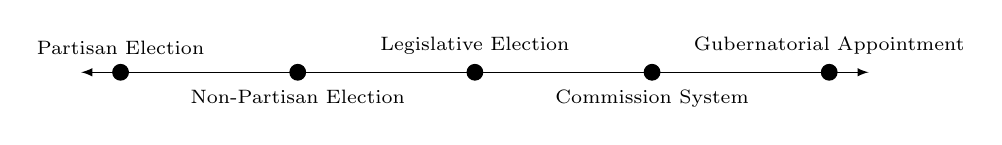
\begin{tikzpicture}
	% a straight line segment
	\draw[latex-latex] (-0.5,0) -- (9.5,0);
	%% the labels
	\node[fill=black,draw=black,circle,inner sep=2pt,label=above:{\scriptsize Gubernatorial Appointment}] at (9,0) {};
	\node[fill=black,draw=black,circle,inner
	sep=2pt,label=below:{\scriptsize Commission System}] at (6.75,0) {};
	\node[fill=black,draw=black,circle,inner
	sep=2pt,label=above:{\scriptsize Legislative Election}] at (4.5,0) {};
	\node[fill=black,draw=black,circle,inner
	sep=2pt,label=below:{\scriptsize Non-Partisan Election}] at (2.25,0) {};
	\node[fill=black,draw=black,circle,inner sep=2pt,label=above:{\scriptsize Partisan Election}] at (0,0) {};
	\end{tikzpicture}
\end{figure} 

\subsection*{Selection Method}
The method of judicial selection is probably the most important variable in determining judicial independence. There are five primary selection methods in use in the United States: executive appointment, legislative appointment, merit selection, non-partisan election, and partisan election. Some states use a mix of these methods; Michigan and Ohio for example, both employ systems which blend partisan primaries with nonpartisan general elections.\footnote{Following normal practice in this field, these states are coded as non-partisan \citep{Canes-Wrone2012, Caldarone2009}, however Tiede \citeyearpar{Tiede2006} does the opposite and codes them as partisan states. Nelson, Caufield, and Martin \citeyearpar{Nelson2013} discuss this coding decision at length.  In accordance with recommendations made in their article, this model will be conducted both ways and examined for differences, with theoretical justifications for both methods made clear.}    Under \citet{Hall2007}'s theory of judicial accountability, I consider executive and legislative appointments to be the most independent/least accountable of the selection methods.  For the majority of states, executive appointment was the original method of appointment.  \footnote{In all executive and legislative appointment states, the Governor is the final appointing authority.  In all executive and legislative appointment states, judges require a confirmation vote of one or both houses of the state legislature.}  Figure \ref{selectioncontinuum} shows how these methods map on to a single dimension continuum with the most accountable method on the left and the most independent method on the right. 

\begin{figure}[tbh]\centering\caption{Current Judicial Selection Methods}\label{selectionmap}
	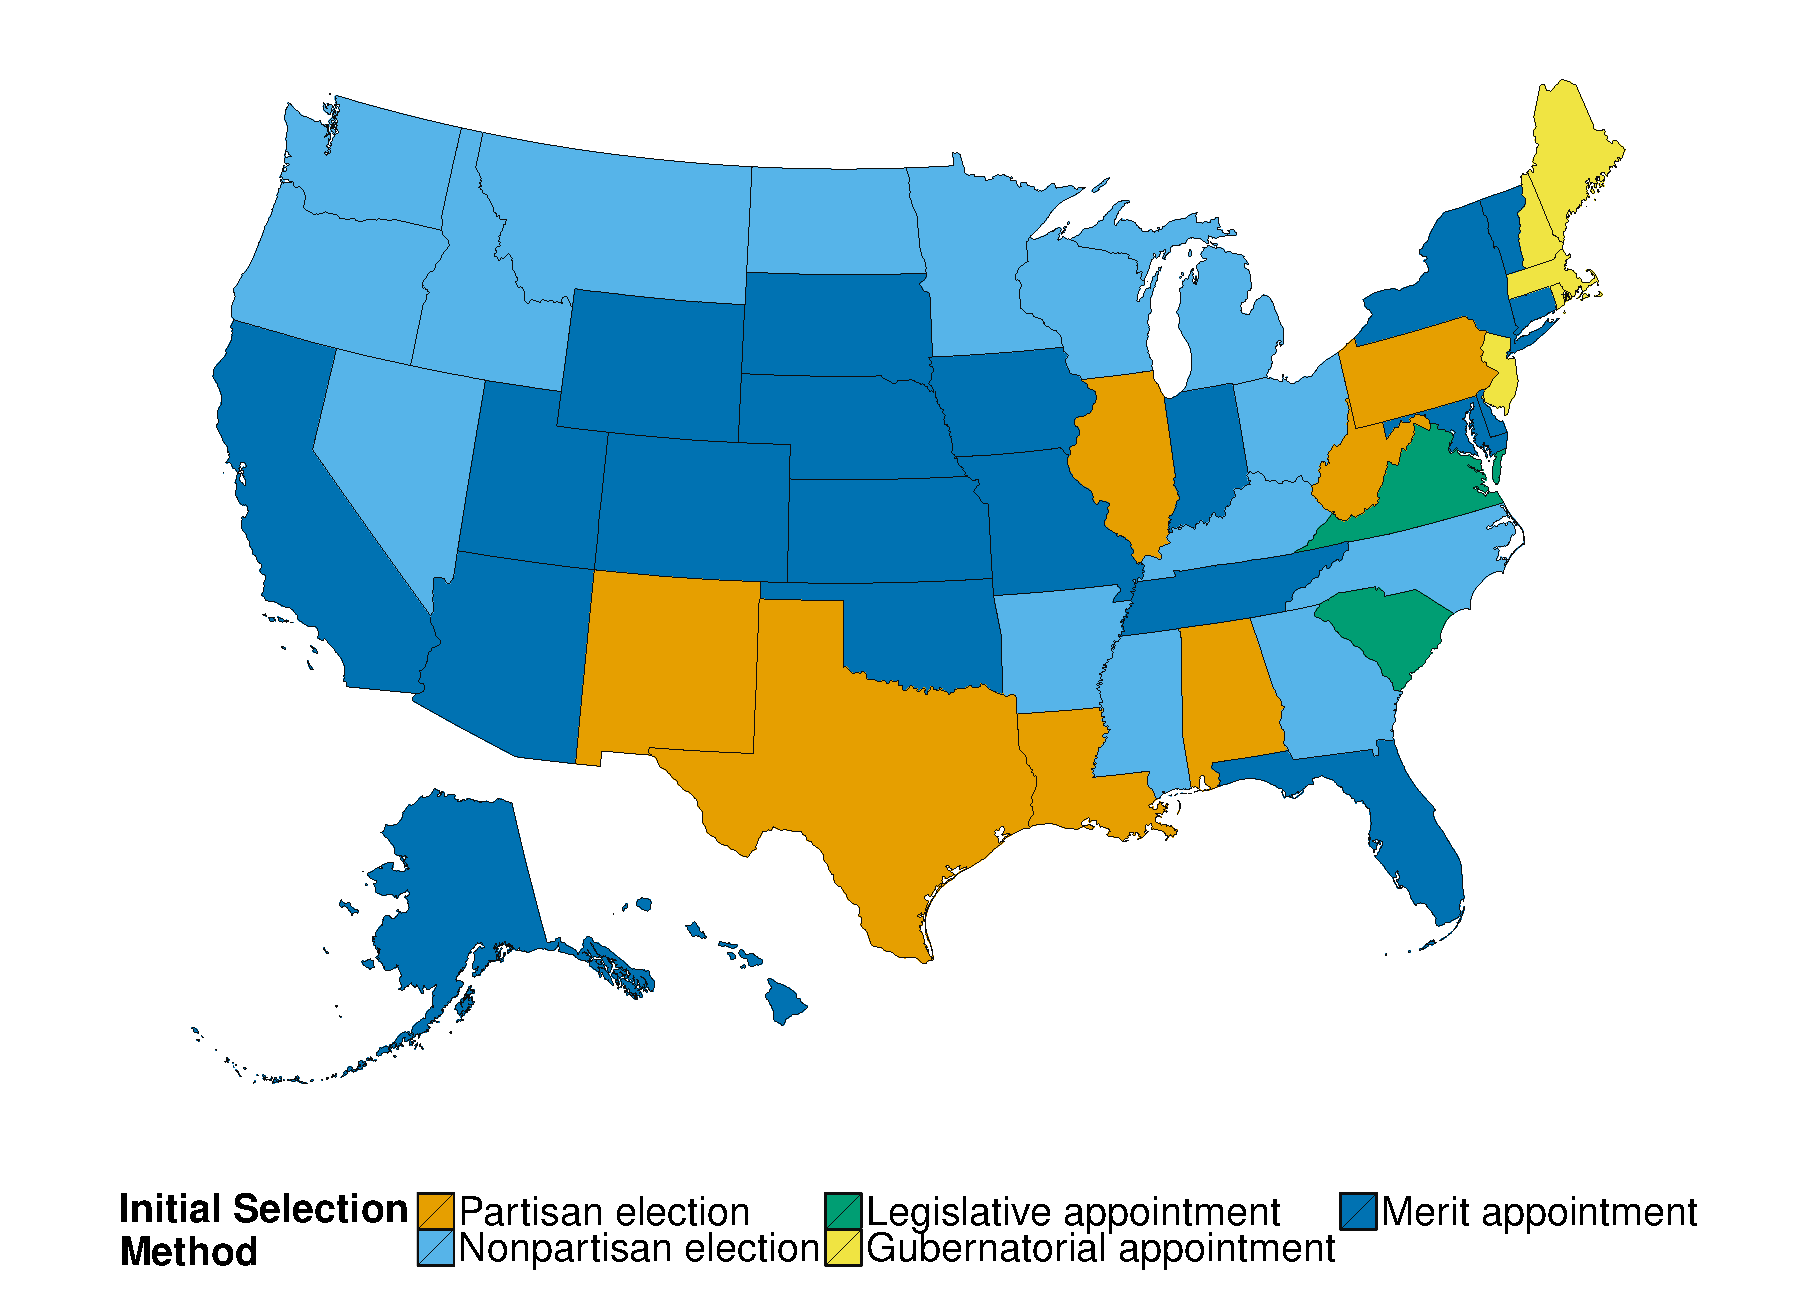
\includegraphics[scale=.5]{graphics/colr_select.pdf}
\end{figure}

The second type of selection system is the Commission System or “merit selection.” The commission system plan came about with the adoption of the Missouri Nonpartisan Court Plan in 1940 \citep{Watson1969}. This system was created with the goal of removing partisanship in judicial selection. This system created a judicial nominating commission who reviews applications and interviews candidates judicial posts. The commission consists of three lawyers selected by the Missouri Bar Association, and three citizens selected by the governor as well as the Chief Justice of the Missouri Supreme Court who serves as the chair of the commission. When a vacancy exists in the courts, the commission submits three names to the Governor who then selects one nominee which is confirmed by the State Senate. Once the judge has completed at least one year in office they stand for retention election. Retention elections are on separate ballots and only ask the voter to vote whether the judge should be retained. This description of the Missouri Plan is representative of the other twenty states which use similar systems.  There is no partisan affiliation listed on the ballot \citep{Watson1969}.  The most substantive difference between commission systems and other systems is the attempt to remove partisanship completely. Appointment, as well as partisan elections, are both acknowledged to be partisan acts, while proponents of commission systems and non-partisan elections claim that these systems eliminate partisanship from judicial selection. 

There are two types of electoral selection: partisan and non-partisan.  Electoral systems are considered to be the least independent due to the number of actors involved in the selection process \citep{Choi2010}. These judges are also generally forced to raise money for advertising and other campaign related expenses.  Debate exists about the ethical implications of raising this money from businesses, interest groups, and litigators that may appear before these judges.\footnote{For empirical evidence of this see \citep{Gibson2008}.}  Elected judges are selected by the electorate in statewide elections.  \citet{Caldarone2009} puts forth the view that when electing judges, the public will elect the judges that most closely match their own personal preferences.  However \citet{Debow2013} states that ``non-partisan judicial elections do not compare favorably with partisan judicial elections'' because the former inhibit the voters ability to make informed decisions.

\subsection*{Retention Method}
Creation of retention elections were a hallmark of the merit selection plan created in Missouri. Retention elections differ from partisan and non-partisan elections in that there is only one candidate involved in the election. As \citeauthor{Reid1999} summarizes: \begin{quote}``Judicial retention elections are intended to preserve the court’s role as an impartial and detached resolver of disputes by ensuring that judges can retain their seats without engaging in the fund raising, politicking, and electioneering that characterize political elections and the political process,'' \citep[68]{Reid1999}.\end{quote}  Retention elections simply ask voters to approve or disapprove of the judge in office. Ballots questions usually appear in the form of: ``Shall each of the persons listed be retained in office as Judge of the Appellate Court, First Judicial District?''

All but the four states which have life or quasi-life terms employ some manner of retention elections. Some states use retention elections such as those listed above. Others use the same type of partisan or non-partisan election as they use for their initial selection. No state uses a commission system then requires the judge to run in a contested election.\footnote{The exception to this is in the case of a judicial vacancy.  If a judge resigns, or dies in office, states have selection mechanisms in place that can differ from the official selection system.  For example, in the case of New Mexico ``All judicial vacancies are filled by the governor from a list of candidates recommended by a judicial nominating commission. The appointee must then compete in a partisan election at the next general election to serve the remainder of the unexpired term'' \citep{AJS}.}  Also no states utilizes a partisan election for initial selection and then uses non-partisan elections for retention.  Contested elections, whether partisan or non-partisan, are considered to be the least independent \citep{Choi2010,ABA2003,Canes-Wrone2012}. Judges who do not face any electoral accountability are considered the most independent in this context.

\begin{figure}[tbh]\centering\caption{Retention Method Independence Space}\label{retentioncontinuum}
	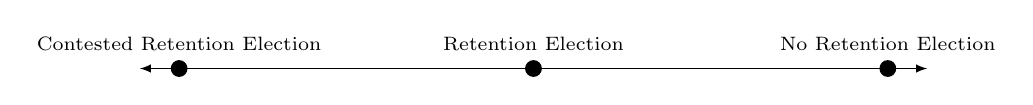
\begin{tikzpicture}
	% a straight line segment
	\draw[latex-latex] (-0.5,0) -- (9.5,0);
	%% the labels
	\node[fill=black,draw=black,circle,inner sep=2pt,label=above:{\scriptsize No Retention Election}] at (9,0) {};
	\node[fill=black,draw=black,circle,inner
	sep=2pt, label=above:{\scriptsize Retention Election}] at (4.5,0) {};
	\node[fill=black,draw=black,circle,inner sep=2pt,label=above:{\scriptsize Contested Retention Election}] at (0,0) {};
	\end{tikzpicture}
\end{figure}

Retention elections are admittedly only a matter of degrees more or less independent than contested elections. Figure \ref{retentioncontinuum} shows how methods of retention can map on to the judicial Independence Continuum.  There is still some debate on whether retention elections create a more independent judiciary. The ABA defends its position that retention elections are more independent and recommends them for all states that utilize elections to retain judges \citep{ABA2003}.  \citep{Canes-Wrone2012} take a divergent position and posit that judges are susceptible to losing their seats based on only one or two salient decisions and also susceptible to attacks from single-issue groups.  This occurred in 2010 when three justices on the Iowa Supreme Court were ousted. These justices had voted to strike down Iowa’s ban on same-sex marriage. There was a prolonged campaign by single-issue groups opposed to same-sex marriage resulting in the judges removal \citep{Iowa2010}.

\subsection*{Term Lengths}
The length of a judicial term is another important factor in determining the level of judicial independence.  In many commission system states seats are vacated by either promotion, retirement, or death. Replacement judges are then appointed to fill out the unexpired terms. The initial term lengths for the new judges in those states range from appointment until the next general election, or from appointment through the remainder of the full term. Subsequent term length is the length of the terms after the initial term. For most elective states this is the same as the initial term length, and for retention states, this the length of a standard term. Term lengths for initial terms range from one year to fourteen years\footnote{While there are four states which have lifetime or quasi-lifetime (age limited terms) only New Jersey requires reappointment after an initial term.} while subsequent terms range from six years to lifetime terms.\footnote{Many states also have statutory term lengths also utilize a mandatory retirement age.}  These term lengths can be compared to U.S. House of Representatives terms which are two years, and U.S. Senate terms which are six years.  The longer that a term is, the more independent choices a judge can make before being held accountable prior to an election.  Figure \ref{termcontinuum} shows how varying term lengths map on to the Independence Continuum.  According to \citet[31]{Rios2006} ``terms must be long enough to reduce the vulnerability of Supreme Court judges.  Tenure need not be for life, but if it coincides with that of appointing authorities then there is the potential for abuse.''\footnote{\citet{Rios2006} uses a binary coding scheme in his study, coding a term length as independent if it was longer than the appointing authority.}  As Hall and others show, most of strategic voting of judges is done in the year prior to an election \citep{Hall1987,Hall1985,Brace2008,Canes-Wrone2012}.  

\begin{figure}[tbh]\centering\caption{Term Length Independence Space}\label{termcontinuum}
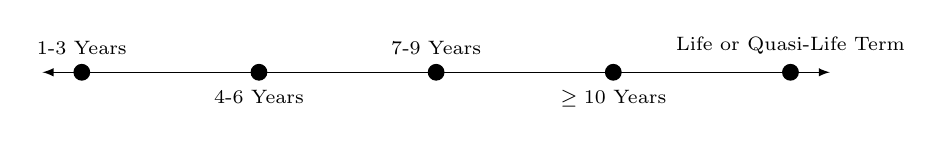
\begin{tikzpicture}
% a straight line segment
\draw[latex-latex] (-0.5,0) -- (9.5,0);
%% the labels
\node[fill=black,draw=black,circle,inner sep=2pt,label=above:{\scriptsize Life or Quasi-Life Term}] at (9,0) {};
\node[fill=black,draw=black,circle,inner
sep=2pt,label=below:{\scriptsize $\geq10$ Years}] at (6.75,0) {};
\node[fill=black,draw=black,circle,inner
sep=2pt,label=above:{\scriptsize 7-9 Years}] at (4.5,0) {};
\node[fill=black,draw=black,circle,inner
sep=2pt,label=below:{\scriptsize 4-6 Years}] at (2.25,0) {};
\node[fill=black,draw=black,circle,inner sep=2pt,label=above:{\scriptsize 1-3 Years}] at (0,0) {};
\end{tikzpicture}	
\end{figure}

There are several arguments for the inclusion of term length as an indicator of judicial independence. The ABA views the term length question as a matter of experience in that lawyers who are experienced and qualified will be reluctant to leave successful private practices if they are forced to return to the job market after only a few years \citep[97]{ABA2003}.   The argument against longer terms is that longer terms provide less opportunity for accountability. The ABA recommends an actively enforced judicial discipline system, which will ensure accountability for systems that do not rely on re-selection stating that judges should only be removed for ``cause'' \citep[103]{ABA2003}.\footnote{This is in reference to an ethical or criminal violation, rather than a punitive punishment as the result of an opinion.  The clearest example of this would be the Iowa case where judges were ousted based on an ideological view, rather than as a breach of ethics or the law.}  The low level of judicial turnover disputes this point of view. In 2012, only 6 of the judges on state supreme courts were not retained. For the years 1964-1998, there were 4,588 retention elections with only 52 judges being voted out of office \citep{Aspin2000}.  

There are several arguments for a connection between longer term lengths and increased judicial independence as well as alternatives such as limiting judges to only a single term. A single term would obviate the need for reappointment or campaigning for their next term \citep{Carrington1998}.  Former Presiding Judge of the Texas Court of Criminal Appeals Morris Overstreet has stated ``if you don't have to go back and face the voters, you don't have to worry about how they're going to retaliate or if they're going to retaliate'' \citep{ABA2003}.  This has the drawback of returning judges to private practice, which may have an effect on their decisions made while on the bench.  No state currently has adopted this practice.

\citet{Hall1987a}'s study of the Louisiana Supreme Court shows that when faced with electoral accountability, the judges have a tendency to avoid casting votes on unpopular issues. Hall concludes that this system ``does not present the opportunity for the unfettered exercise of individual preferences'' \citep[46]{Hall1987a}.  Hall also concludes that justices who perceive themselves to have views inconsistent with public opinion,  and who desire to keep their jobs, may be hesitant to publish opinions which are against public opinion. Hall states that ``whether voters and opponents are cognizant of the justices’ behavior or not, certain justices seem to fear the prospect of electoral sanction and consequently alter their behavior'' \citep[1123]{Hall1987b}.  While voters’ knowledge of justices' records is questionable, certainly the judges' actions are not.  As Hall shows, judges act as if voter's will have knowledge of their records and vote strategically to minimize the electoral losses they may suffer.

\subsection*{Docket Control}
The ability of a court to control its own docket is another important factor in examining \textit{de jure} independence.  Docket control comes in many forms, ranging from complete discretionary control, as in the case of the U.S. Supreme Court, which can grant or deny any appellate case that it wishes to hear with few exceptions, to states such as Wyoming which have no intermediate appellate courts, and therefore has very little control over its appellate docket. There are also many states which have mandatory appeals on certain subject matter or litigants, and discretionary appeals on other types of cases.  Typically, docket control is set through statues passed by the state legislature, similar to the appellate jurisdiction of the U.S. Supreme Court, although some states have their docket discretion set through the state constitution.\footnote{Death penalty cases are an exception to this general rule.  In many cases death penalty appeals must be heard by the Court of Last Resort for that state, and this reduces the court's discretion in these cases.  In the case of this analysis, this exception will be ignored.  For states which utilize complete discretionary docket control except for death penalty cases, they will be coded as having complete discretion.}

\begin{figure}[tbh]\centering\caption{Docket Control Independence Space}\label{docketcontinuum}
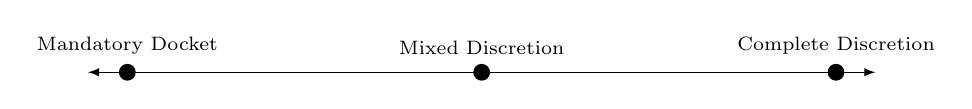
\begin{tikzpicture}
% a straight line segment
\draw[latex-latex] (-0.5,0) -- (9.5,0);
%% the labels
\node[fill=black,draw=black,circle,inner sep=2pt,label=above:{\scriptsize Complete Discretion}] at (9,0) {};
\node[fill=black,draw=black,circle,inner
sep=2pt,label=above:{\scriptsize Mixed Discretion}] at (4.5,0) {};
\node[fill=black,draw=black,circle,inner sep=2pt,label=above:{\scriptsize Mandatory Docket}] at (0,0) {};
\end{tikzpicture}
\end{figure}

The ability of a court to control its docket has multiple facets to it's effect on independence.  The first is that if a court has control over its docket, then the workload of the court can be reduced to only those cases that the court wishes to make a statement on, rather than hearing every case, including those on which there is already clear precedent \citep{Maltzman2000}.  Also, reduced workload enables a court to spend more time on those cases that it deems important.  While this may seem more related to efficiency than independence, the two are inter-connected in this case.  As Squire notes, the ability to pick and choose cases allows an appellate court to craft their decisions more carefully than a court which has no discretion \citep{Squire2008}.

The second aspect of docket control on judicial independence stems directly from the first.  Not only can judges spend more time on cases under a discretionary docket, but they can pick and choose the cases that they want to issue an opinion on.  As Fontana notes, this can be very important to both the influence and the legitimacy of a court \citep{Fontana2011}.  Fontana notes that had the \textit{Brown v. Board of Education} decision been decided ten years earlier, it might not have had the effect that it had, due to a lack of support from the President, and antipathy from southern states, and their representatives in Congress.  This is supported by \citet{Rosenberg1991} in light of the very extensive process to bring the country in to compliance with the Court's ruling in \textit{Brown}.  Had this process happened earlier, there might have been no compliance, causing both extended oppression of African-Americans in the South, as well as a severe blow to the legitimacy of the Court.  Fontana refers to this as ``legitimacy timing'' \citep[627]{Fontana2011}.  

Another important aspect of docket control is the effect that it has on a judge's voting preferences.  Whether following a strictly legal interpretation, or an ideological preferences, a key part of judicial independence is a judge's ability to vote her preferences.  Songer et al. note that when courts have discretionary control over their dockets, the judges are much more likely to follow the attitudinal model of voting preferences \citep{Songer2003}.  This would lead us to believe that discretionary control allows more freedom in the preferences that judges exercise in this case.   This is also supported by Melinda Gann Hall's study of the Louisiana Supreme Court.  Hall finds that in discretionary cases, there is a significant number of dissents, rather than in mandatory cases, which shows much more unanimous decisions \citep{Hall1985}.  There are several hypotheses for this outcome, chiefly that under mandatory review, there are many more ``easy'' cases.  That is cases which have a clear precedent and had no complex legal complications.  These cases could have been successfully disposed of by the lower courts, but were required to be heard by the state supreme court.   

The most important aspect of a court's jurisdictional control comes from their independence from the executive and legislature.  This is especially a concern when the government is a party to a case that the court could potentially hear.  As \citet[6]{Rios2014} note, ``Indeed, a court that offers little constraint on government can appear to be highly constraining if it chooses its cases wisely. It certainly can ensure systematic compliance, which makes inferring judicial influence from the outcomes of legal conflicts difficult.''  They also posit that judicial decision making can appear to be independent if the court removes contentious cases from its docket.  The example of same-sex marriage can illustrate this quite clearly.  Had the Iowa Supreme Court simply chosen to uphold the lower court ruling in \cite{iowagay}, they most likely could have avoided the lengthy campaign that was mounted against the retention of three justices that ultimately resulted in their dismissal.

%\singlespacing
%\bibliographystyle{apsr}
%\bibliography{measurementbib}	
\end{document}